\documentclass[12pt, a4paper]{report}

%%%%%%%%%%%%%%%%%%%%%%%%%%%%%%%%%
% PACKAGE IMPORTS
%%%%%%%%%%%%%%%%%%%%%%%%%%%%%%%%%

% \usepackage[sfdefault]{roboto}
% \usepackage[T1]{fontenc}
% \usepackage[utf8]{inputenc}

\usepackage[tmargin=3cm,rmargin=1in,lmargin=1in,margin=0.85in,bmargin=3cm]{geometry}
\usepackage{amsmath,amsfonts,amsthm,amssymb,mathtools}
\usepackage{diffcoeff} 
\usepackage{xfrac}
\usepackage[makeroom]{cancel}
\usepackage{bookmark}
\usepackage{enumitem}
\usepackage{hyperref,theoremref}
\hypersetup{
	colorlinks=true,
  allcolors=fg,
	bookmarksnumbered=true,
	bookmarksopen=true
}
\usepackage[most,many,breakable]{tcolorbox}
\usepackage{xcolor}
\usepackage{varwidth}
\usepackage{etoolbox}
\usepackage{nameref}
\usepackage{multicol,array}
\usepackage{tikz-cd}
\usepackage{algorithm}
\usepackage{algpseudocode}
%\usepackage[ruled,vlined,linesnumbered]{algorithm2e}
\usepackage{booktabs}
\usepackage{comment}
\usepackage{import}
\usepackage{xifthen}
\usepackage{pdfpages}
\usepackage{transparent}
\usepackage{caption}
\usepackage{marginnote}
\usepackage{float}
\usepackage{tikz}
\usepackage{tikzsymbols}
\usetikzlibrary{patterns, shapes.misc}
\usepackage{pgfplots}
\pgfplotsset{compat=1.18}
\usepackage{xpatch}% to patch \cancel
\usepackage{forest}

% \usepackage{graphicx}
% \graphicspath{ {./images/} }

\makeatletter
\xpatchcmd{\canto@vector}{\vector}{\line}{}{}
\makeatother

% removing algorithm numbering
\renewcommand{\thealgorithm}{}

% don't know what this is
% \newcommand\mycommfont[1]{\footnotesize\ttfamily\textcolor{blue}{#1}}
% \SetCommentSty{mycommfont}
% \newcommand{\incfig}[1]{%
%     \def\svgwidth{\columnwidth}
%     \import{./figures/}{#1.pdf_tex}
% }

\newcommand{\tikzmark}[1]{\tikz[overlay,remember picture] \node (#1) {};}

\tikzset{cross/.style={cross out, draw=black, minimum size=2*(#1-\pgflinewidth), inner sep=0pt, outer sep=0pt}, cross/.default={4.5pt}}

\forestset{
  declare toks={elo}{}, % Edge Label Options
  anchors/.style={anchor=#1,child anchor=#1,parent anchor=#1},
  dot/.style={tikz+={\fill (.child anchor) circle[radius=#1];}},
  dot/.default=2pt,
  decision edge label/.style n args=3{
    edge label/.expanded={node[midway,auto=#1,anchor=#2,\forestoption{elo}]{\strut$\unexpanded{#3}$}}
  },
  decision/.style={if n=1
    {decision edge label={left}{north}{#1}}
    {decision edge label={right}{south}{#1}}
  },
  decision tree/.style={
    for tree={
      grow=east,
      calign angle=45,
      calign=fixed edge angles,
      s sep=0.5em,l=4ex,
      if n children=0{anchors=south}{
        if n=1{anchors=north}{anchors=south}},
      math content,
    },
    anchors=east, outer sep=2pt,
    delay={for descendants={split option={content}{;}{content,decision}}},
  },
    decision tree nodes/.style={
    for tree={
      grow=east,
      calign angle=45,
      calign=fixed edge angles,
      s sep=0.5em,l=4ex,
      if n children=0{anchors=west}{
        if n=1{anchors=north}{anchors=south}},
      math content,
    },
    anchors=east, outer sep=2pt,
    dot=2pt,for descendants=dot,
    delay={for descendants={split option={content}{;}{content,decision}}},
  },
}

% \renewcommand\qedsymbol{$\Laughey$}   %uncomment to use smile as qedsymbol


%%%%%%%%%%%%%%%%%%%%%%%%%%%%%%
% COLORS
%%%%%%%%%%%%%%%%%%%%%%%%%%%%%%

\definecolor{bg}{HTML}{F2F2F2}
\definecolor{fg}{HTML}{282828}


%%%%%%%%%%%%%%%%%%%%%%%%%%%%
% MARGINS
%%%%%%%%%%%%%%%%%%%%%%%%%%%%

\setlength{\parindent}{0pt}

% change default chapter distance
\makeatletter
% --- Patch \chapter
\patchcmd{\@makechapterhead}{50\p@}{\chapheadtopskip}{}{}% Space from top of page to CHAPTER X
\patchcmd{\@makechapterhead}{20\p@}{\chapheadsep}{}{}% Space between CHAPTER X and CHAPTER TITLE
\patchcmd{\@makechapterhead}{40\p@}{\chapheadbelowskip}{}{}% Space between CHAPTER TITLE and text
% --- Patch \chapter*
\patchcmd{\@makeschapterhead}{50\p@}{\chapheadtopskip}{}{}% Space from top of page to CHAPTER TITLE
\patchcmd{\@makeschapterhead}{40\p@}{\chapheadbelowskip}{}{}% SPace between CHAPTER TITLE and text
\makeatother
% Set new lengths
\newlength{\chapheadtopskip}\setlength{\chapheadtopskip}{0pt}
\newlength{\chapheadsep}\setlength{\chapheadsep}{15pt}
\newlength{\chapheadbelowskip}\setlength{\chapheadbelowskip}{25pt}

%================================
% THEOREM BOX
%================================
\tcbuselibrary{theorems,skins,hooks}
\newtcbtheorem[number within=chapter]{Theorem}{Theorem}
{%
	enhanced,
	breakable,
	colback = bg,
	frame hidden,
	boxrule = 0sp,
	borderline west = {2pt}{0pt}{fg!85!bg},
	sharp corners,
	detach title,
	before upper = \tcbtitle\par\smallskip,
	coltitle = fg!85!bg,
	fonttitle = \sffamily,
	description font = \mdseries,
	separator sign none,
	segmentation style={solid, fg},
}
{th}
\tcbuselibrary{theorems,skins,hooks}
\newtcbtheorem[number within=chapter]{theorem}{Theorem}
{%
	enhanced,
	breakable,
	colback = bg,
	frame hidden,
	boxrule = 0sp,
	borderline west = {2pt}{0pt}{fg!85!bg},
	sharp corners,
	detach title,
	before upper = \tcbtitle\par\smallskip,
	coltitle = fg!85!bg,
	fonttitle = \sffamily,
	description font = \mdseries,
	separator sign none,
	segmentation style={solid, fg},
}
{th}


%================================
% Corollary
%================================
\tcbuselibrary{theorems,skins,hooks}
\newtcbtheorem[number within=chapter]{Corollary}{Corollary}
{%
	enhanced,
	breakable,
	colback = bg,
	frame hidden,
	boxrule = 0sp,
	borderline west = {2pt}{0pt}{fg!70!bg},
	sharp corners,
	detach title,
	before upper = \tcbtitle\par\smallskip,
	coltitle = fg!70!bg,
	fonttitle = \sffamily,
	description font = \mdseries,
	separator sign none,
	segmentation style={solid, fg},
}
{th}
\tcbuselibrary{theorems,skins,hooks}
\newtcbtheorem[number within=chapter]{corollary}{Corollary}
{%
	enhanced,
	breakable,
	colback = bg,
	frame hidden,
	boxrule = 0sp,
	borderline west = {2pt}{0pt}{fg!70!bg},
	sharp corners,
	detach title,
	before upper = \tcbtitle\par\smallskip,
	coltitle = fg!70!bg,
	fonttitle = \sffamily,
	description font = \mdseries,
	separator sign none,
	segmentation style={solid, fg},
}
{th}

%================================
% LEMMA
%================================
\tcbuselibrary{theorems,skins,hooks}
\newtcbtheorem[number within=chapter]{Lemma}{Lemma}
{%
	enhanced,
	breakable,
	colback = bg,
	frame hidden,
	boxrule = 0sp,
	borderline west = {2pt}{0pt}{fg!70!bg},
	sharp corners,
	detach title,
	before upper = \tcbtitle\par\smallskip,
	coltitle = fg!70!bg,
	fonttitle = \sffamily,
	description font = \mdseries,
	separator sign none,
	segmentation style={solid, fg},
}
{th}
\tcbuselibrary{theorems,skins,hooks}
\newtcbtheorem[number within=chapter]{lemma}{Lemma}
{%
	enhanced,
	breakable,
	colback = bg,
	frame hidden,
	boxrule = 0sp,
	borderline west = {2pt}{0pt}{fg!70!bg},
	sharp corners,
	detach title,
	before upper = \tcbtitle\par\smallskip,
	coltitle = fg!70!bg,
	fonttitle = \sffamily,
	description font = \mdseries,
	separator sign none,
	segmentation style={solid, fg},
}
{th}

%================================
% PROPERTY
%================================
\tcbuselibrary{theorems,skins,hooks}
\newtcbtheorem[number within=chapter]{Prop}{Property}
{%
	enhanced,
	breakable,
	colback = bg,
	frame hidden,
	boxrule = 0sp,
	sharp corners,
	detach title,
	before upper = \tcbtitle\par\smallskip,
	coltitle = fg,
	fonttitle = \sffamily,
	description font = \mdseries,
	separator sign none,
	segmentation style={solid, fg},
}
{th}
\tcbuselibrary{theorems,skins,hooks}
\newtcbtheorem[number within=chapter]{prop}{Property}
{%
	enhanced,
	breakable,
	colback = bg,
	frame hidden,
	boxrule = 0sp,
	sharp corners,
	detach title,
	before upper = \tcbtitle\par\smallskip,
	coltitle = fg,
	fonttitle = \sffamily,
	description font = \mdseries,
	separator sign none,
	segmentation style={solid, fg},
}
{th}


%================================
% CLAIM
%================================
\tcbuselibrary{theorems,skins,hooks}
\newtcbtheorem[number within=chapter]{claim}{Claim}
{%
	enhanced,
	breakable,
	colback = bg,
	frame hidden,
	boxrule = 0sp,
	borderline west = {2pt}{0pt}{fg},
	sharp corners,
	detach title,
	before upper = \tcbtitle\par\smallskip,
	coltitle = fg,
	fonttitle = \sffamily,
	description font = \mdseries,
	separator sign none,
	segmentation style={solid, fg},
}
{th}

%================================
% Exercise
%================================
\tcbuselibrary{theorems,skins,hooks}
\newtcbtheorem[number within=chapter]{Exercise}{Exercise}
{%
	enhanced,
	breakable,
	colback = bg,
	frame hidden,
	boxrule = 0sp,
	sharp corners,
	detach title,
	before upper = \tcbtitle\par\smallskip,
	coltitle = fg,
	fonttitle = \sffamily,
	description font = \mdseries,
	separator sign none,
	segmentation style={solid, fg},
}
{th}
\tcbuselibrary{theorems,skins,hooks}
\newtcbtheorem[number within=chapter]{exercise}{Exercise}
{%
	enhanced,
	breakable,
	colback = bg,
	frame hidden,
	boxrule = 0sp,
	sharp corners,
	detach title,
	before upper = \tcbtitle\par\smallskip,
	coltitle = fg,
	fonttitle = \sffamily,
	description font = \mdseries,
	separator sign none,
	segmentation style={solid, fg},
}
{th}

%================================
% EXAMPLE BOX
%================================

\newtcbtheorem[number within=chapter]{Example}{Example}
{%
	enhanced,
	breakable,
	colback = bg,
	frame hidden,
	boxrule = 0sp,
	sharp corners,
	detach title,
	before upper = \tcbtitle\par\smallskip,
	coltitle = fg,
	fonttitle = \sffamily,
	description font = \mdseries,
	separator sign none,
	segmentation style={solid, fg},
}
{ex}
\newtcbtheorem[number within=chapter]{example}{Example}
{%
	enhanced,
	breakable,
	colback = bg,
	frame hidden,
	boxrule = 0sp,
	sharp corners,
	detach title,
	before upper = \tcbtitle\par\smallskip,
	coltitle = fg,
	fonttitle = \sffamily,
	description font = \mdseries,
	separator sign none,
	segmentation style={solid, fg},
}
{ex}


%================================
% DEFINITION BOX
%================================

\tcbuselibrary{theorems,skins,hooks}
\newtcbtheorem[number within=chapter]{Definition}{Definition}
{%
	enhanced,
	breakable,
	colback = bg,
	frame hidden,
	boxrule = 0sp,
	borderline west = {2pt}{0pt}{fg},
	sharp corners,
	detach title,
	before upper = \tcbtitle\par\smallskip,
	coltitle = fg,
	fonttitle = \sffamily,
	description font = \mdseries,
	separator sign none,
	segmentation style={solid, fg},
}
{def}
\tcbuselibrary{theorems,skins,hooks}
\newtcbtheorem[number within=chapter]{definition}{Definition}
{%
	enhanced,
	breakable,
	colback = bg,
	frame hidden,
	boxrule = 0sp,
	borderline west = {2pt}{0pt}{fg},
	sharp corners,
	detach title,
	before upper = \tcbtitle\par\smallskip,
	coltitle = fg,
	fonttitle = \sffamily,
	description font = \mdseries,
	separator sign none,
	segmentation style={solid, fg},
}
{def}

%================================
% QUESTION BOX
%================================

\makeatletter
\newtcbtheorem{question}{Question}
{%
	enhanced,
	breakable,
	colback = bg,
	frame hidden,
	boxrule = 0sp,
	borderline = {0.5pt}{0pt}{fg},
	rounded corners,
	detach title,
	before upper = \tcbtitle\par\smallskip,
	coltitle = fg,
	fonttitle = \sffamily,
	description font = \mdseries,
	separator sign none,
	segmentation style={solid, fg},
}
{def}
\makeatother

%================================
% SOLUTION BOX
%================================

\makeatletter
\newtcbtheorem{solution}{Solution}
{%
	enhanced,
	breakable,
	colback = bg,
	frame hidden,
	boxrule = 0sp,
	borderline west = {2pt}{0pt}{fg},
	sharp corners,
	detach title,
	before upper = \tcbtitle\par\smallskip,
	coltitle = fg,
	fonttitle = \sffamily,
	description font = \mdseries,
	separator sign none,
	segmentation style={solid, fg},
}
{def}
\makeatother

%================================
% NOTE BOX
%================================

\usetikzlibrary{arrows,calc,shadows.blur}
\tcbuselibrary{skins}
\newtcolorbox{note}[1][]{%
	enhanced jigsaw,
	colback=bg,
	colframe=fg,
	size=small,
	boxrule=1pt,
  title=\textbf{\textbf{NOTE:}},
	before upper = \tcbtitle\par,
	detach title,
	coltitle=fg,
	breakable,
	drop shadow=fg!50!bg,
	#1,
}

%================================
% EXAM EXERCISE
%================================

\tcbuselibrary{theorems}
\newtcolorbox[auto counter]{examexercise}[1][]{%
  colback = white,
  colbacktitle = white,
  coltitle = black,
  center title,
	frame hidden,
	colframe = white,
	boxrule = 0sp,
  fonttitle = \sffamily,
  title={\textbf{Exercise \thetcbcounter}},
  #1,
}

%%%%%%%%%%%%%%%%%%%%%%%%%%%%%%
% SELF MADE COMMANDS
%%%%%%%%%%%%%%%%%%%%%%%%%%%%%%


% non numbered
\newcommand{\dfn}[2]{\begin{definition*}{#1}{}#2\end{definition*}}
\newcommand{\thm}[2]{\begin{theorem*}{#1}{}#2\end{theorem*}}
\newcommand{\cor}[2]{\begin{corollary*}{#1}{}#2\end{corollary*}}
\newcommand{\lem}[2]{\begin{lemma*}{#1}{}#2\end{lemma*}}
\newcommand{\pro}[2]{\begin{prop*}{#1}{}#2\end{prop*}}
\newcommand{\clm}[3]{\begin{claim*}{#1}{#2}#3\end{claim*}}
\newcommand{\exs}[3]{\begin{exercise*}{#1}{#2}#3\end{exercise*}}
\newcommand{\exa}[2]{\begin{example*}{#1}{}#2\end{example*}}
\newcommand{\qs}[2]{\begin{question*}{#1}{}#2\end{question*}}
\newcommand{\sol}[2]{\begin{solution*}{#1}{}#2\end{solution*}}
\newcommand{\prf}[2]{\begin{myproof}{#1}{}#2\end{myproof}}
\newcommand{\nt}[1]{\begin{note}#1\end{note}}

% numbered
\newcommand{\ndfn}[2]{\begin{definition}{#1}{}#2\end{definition}}
\newcommand{\nthm}[2]{\begin{theorem}{#1}{}#2\end{theorem}}
\newcommand{\ncor}[2]{\begin{corollary}{#1}{}#2\end{corollary}}
\newcommand{\nlem}[2]{\begin{lemma}{#1}{}#2\end{lemma}}
\newcommand{\npro}[2]{\begin{prop}{#1}{}#2\end{prop}}
\newcommand{\nclm}[3]{\begin{claim}{#1}{#2}#3\end{claim}}
\newcommand{\nexs}[3]{\begin{exercise}{#1}{#2}#3\end{exercise}}
\newcommand{\nexa}[2]{\begin{example}{#1}{}#2\end{example}}

% exam title
\newcommand{\inlinemaketitle}{{\let\newpage\relax\maketitle}}
\newcommand{\examex}[1]{\begin{examexercise}#1\end{examexercise}}

\newcommand*\circled[1]{\tikz[baseline=(char.base)]{
		\node[shape=circle,draw,inner sep=1pt] (char) {#1};}}
\newcommand\getcurrentref[1]{%
	\ifnumequal{\value{#1}}{0}
	{??}
	{\the\value{#1}}%
}
\newcommand{\getCurrentSectionNumber}{\getcurrentref{section}}
\newenvironment{myproof}[2][\proofname]{%
	\proof[\textnormal{\textbf{PROOF  }}\itshape #2:]$ $\par\nobreak\ignorespaces
}{\endproof}

\newcommand{\mclm}[2]{\begin{myclaim}[#1]#2\end{myclaim}}
\newenvironment{myclaim}[1][\claimname]{\proof[ #1: ]}{}

\newcounter{mylabelcounter}

\makeatletter
\newcommand{\setword}[2]{%
	\phantomsection
	#1\def\@currentlabel{\unexpanded{#1}}\label{#2}%
}
\makeatother


\tikzset{
	symbol/.style={
			draw=none,
			every to/.append style={
					edge node={node [sloped, allow upside down, auto=false]{$#1$}}}
		}
}

% deliminators
\DeclarePairedDelimiter{\abs}{\lvert}{\rvert}
\DeclarePairedDelimiter{\norm}{\lVert}{\rVert}

\DeclarePairedDelimiter{\ceil}{\lceil}{\rceil}
\DeclarePairedDelimiter{\floor}{\lfloor}{\rfloor}
\DeclarePairedDelimiter{\round}{\lfloor}{\rceil}

\newsavebox\diffdbox
\newcommand{\slantedromand}{{\mathpalette\makesl{d}}}
\newcommand{\makesl}[2]{%
\begingroup
\sbox{\diffdbox}{$\mathsurround=0pt#1\mathrm{#2}$}%
\pdfsave
\pdfsetmatrix{1 0 0.2 1}%
\rlap{\usebox{\diffdbox}}%
\pdfrestore
\hskip\wd\diffdbox
\endgroup
}
\newcommand{\dd}[1][]{\ensuremath{\mathop{}\!\ifstrempty{#1}{%
\slantedromand\@ifnextchar^{\hspace{0.2ex}}{\hspace{0.1ex}}}%
{\slantedromand\hspace{0.2ex}^{#1}}}}
\ProvideDocumentCommand\dv{o m g}{%
  \ensuremath{%
    \IfValueTF{#3}{%
      \IfNoValueTF{#1}{%
        \frac{\dd #2}{\dd #3}%
      }{%
        \frac{\dd^{#1} #2}{\dd #3^{#1}}%
      }%
    }{%
      \IfNoValueTF{#1}{%
        \frac{\dd}{\dd #2}%
      }{%
        \frac{\dd^{#1}}{\dd #2^{#1}}%
      }%
    }%
  }%
}
\providecommand*{\pdv}[3][]{\frac{\partial^{#1}#2}{\partial#3^{#1}}}
\DeclareMathOperator{\Lap}{\mathcal{L}}
\DeclareMathOperator{\Var}{Var} % varience
\DeclareMathOperator{\Cov}{Cov} % covarience
\DeclareMathOperator{\E}{E} % expected

\let\oldleq\leq
\let\oldgeq\geq
\renewcommand{\leq}{\leqslant}
\renewcommand{\geq}{\geqslant}


%%%%%%%%%%%%%%%%%%%%%%%%%%%%%%%%%%%%%%%%%%%
% TABLE OF CONTENTS
%%%%%%%%%%%%%%%%%%%%%%%%%%%%%%%%%%%%%%%%%%%

\usepackage{titletoc}
\contentsmargin{0cm}
\titlecontents{part}[-1pc]
{\addvspace{50pt}%
	
\begin{tikzpicture}[remember picture, overlay]%
		\draw[fill=fg!85,draw=fg!85] (-4.5,-0.2) rectangle (-0.15,0.55);%
		\pgftext[left,x=-1.6cm,y=0.15cm]{\color{bg}\Large Part}%
	\end{tikzpicture}\color{fg}\large}
{}
{}
{}
\titlecontents{chapter}[5pc]
{\addvspace{30pt}%
	
\begin{tikzpicture}[remember picture, overlay]%
		\draw[fill=fg!85,draw=fg!85] (-3.6,-0.2) rectangle (-0.12,0.55);%
		\pgftext[left,x=-3.5cm,y=0.15cm]{\color{bg}\Large Chapter\ \thecontentslabel}%
	\end{tikzpicture}\color{fg}\large}%
{}
{}
{\;\titlerule\;\large Page \thecontentspage
	\begin{tikzpicture}[remember picture, overlay]
		\draw[fill=fg,draw=fg] (4pt,0.2pt) rectangle (4,0.2pt);
	\end{tikzpicture}}%
\titlecontents{section}[5pc]
{\addvspace{2pt}}
{\contentslabel[\thecontentslabel]{2pc}}
{}
{\hfill\small \thecontentspage}
[]
\titlecontents{subsection}[5pc]
{\addvspace{2pt}}
{\scriptsize$\bullet$\quad\small}
{}
{\hfill\small}
% {\hfill\small \thecontentspage}
[]

\makeatletter
\renewcommand{\tableofcontents}{%
	\chapter*{%
	  \vspace*{-20\p@}%
	  \begin{tikzpicture}[remember picture, overlay]%
		  \pgftext[right,x=16.7cm,y=0.2cm]{\color{fg!85}\Huge \contentsname}%
		  \draw[fill=fg!85,draw=fg!85] (14.6,-0.65) rectangle (20,1);%
		  \clip (14.6,-0.65) rectangle (20,1);
		  \pgftext[right,x=16.7cm,y=0.2cm]{\color{bg}\Huge \contentsname}%
	  \end{tikzpicture}}%
	\@starttoc{toc}}
\makeatother



\title{\Huge{Implementazione Distribuita dell'Algoritmo Flood-Fill}}
\author{\Large{\textit{Tam Gabriele, Merlo Filippo}}}
\date{\today}

\begin{document}

\maketitle

\newpage
\pdfbookmark[section]{\contentsname}{toc}
\tableofcontents
\pagebreak

\begin{abstract}
  abstract example
\end{abstract}

\chapter{Introduzione}

L'algoritmo \emph{Flood-Fill} è una tecnica ampiamente utilizzata in grafica computerizzata per determinare e riempire un'area connessa in una struttura bidimensionale, come un'immagine digitale. Data una posizione iniziale e un colore di riempimento, l'algoritmo riempie tutti i pixel adiacenti che condividono lo stesso colore iniziale, creando così un'area uniforme.

Nel contesto dei sistemi distribuiti, l'implementazione dell'algoritmo Flood-Fill presenta sfide significative. In particolare, quando ogni pixel dell'immagine è rappresentato da un nodo indipendente in una rete distribuita, emergono problemi legati alla comunicazione tra nodi, alla consistenza dello stato, alla gestione delle richieste concorrenti e alla tolleranza ai guasti.

Questo documento presenta un'analisi dettagliata dell'implementazione distribuita dell'algoritmo Flood-Fill. Verranno esaminati i requisiti funzionali e non funzionali del sistema, le assunzioni fatte e le sfide affrontate. Successivamente, verrà presentata una soluzione progettuale che affronta queste sfide, con particolare attenzione alle scelte implementative e agli algoritmi utilizzati.

\subsection{Descrizione del Problema}

Data un'immagine bidimensionale $img[][]$, dove ogni elemento $img[i][j]$ rappresenta il colore di un pixel, e data la posizione di un pixel $(x, y)$ insieme a un nuovo colore $newColor$, l'obiettivo è sostituire il colore esistente del pixel dato e di tutti i pixel adiacenti (orizzontalmente, verticalmente e diagonalmente) che condividono lo stesso colore con il nuovo colore.

In un sistema distribuito, ogni pixel è rappresentato da un nodo in un grafo, operante come un processo autonomo nella rete. L'obiettivo è garantire che quando un nodo cambia colore, il cambiamento si propaghi correttamente a tutti i nodi adiacenti con lo stesso colore, rispettando i requisiti funzionali e non funzionali del sistema.

\subsection{Terminologia}

Per evitare ambiguità e garantire coerenza nella trattazione, definiamo i seguenti termini chiave che saranno utilizzati nel documento:

\begin{itemize}
    \item \textbf{Nodo}: Un processo autonomo nella rete che rappresenta un singolo pixel dell'immagine.
    \item \textbf{Colore}: Lo stato di un nodo, rappresentante il colore attuale del pixel associato.
    \item \textbf{Cluster}: Un insieme di nodi adiacenti che condividono lo stesso colore.
    \item \textbf{Nodo Leader}: Un nodo designato che gestisce le operazioni e le decisioni per un cluster.
    \item \textbf{Nodi Vicini}: I nodi adiacenti a un nodo dato, connessi tramite relazioni di adiacenza (orizzontale, verticale, diagonale).
    \item \textbf{Cambio di Colore}: L'operazione mediante la quale un nodo (e potenzialmente il suo cluster) cambia il proprio colore.
\end{itemize}

\chapter{Analisi}

In questa sezione vengono elencati i requisiti funzionali e non funzionali del sistema, insieme alle assunzioni e ai vincoli considerati nell'implementazione dell'algoritmo Flood-Fill in un ambiente distribuito.

\subsection{Requisiti Funzionali}

\begin{enumerate}
    \item \textbf{Colorazione Distribuita}: Il sistema deve consentire la colorazione dei nodi in modo distribuito, permettendo a un nodo di cambiare il proprio colore e propagare il cambiamento ai nodi adiacenti che condividono lo stesso colore iniziale.
    \item \textbf{Propagazione del Cambiamento}: Quando un nodo cambia colore, il cambiamento deve propagarsi correttamente attraverso il cluster, assicurando che tutti i nodi adiacenti con lo stesso colore iniziale vengano aggiornati.
    \item \textbf{Gestione di Richieste Concorrenti}: Il sistema deve gestire richieste di cambio colore concorrenti provenienti da nodi diversi, garantendo un comportamento coerente e deterministico.
    \item \textbf{Comunicazione tra Nodi}: I nodi devono poter comunicare tra loro per scambiare informazioni sullo stato e coordinare le operazioni di colorazione.
    \item \textbf{Unione di Cluster}: Il sistema deve essere in grado di gestire la fusione di cluster quando due cluster di colore identico diventano adiacenti a seguito di operazioni di colorazione.
    \item \textbf{Robustezza ai Guasti}: Il sistema deve tollerare il fallimento di nodi individuali senza compromettere la consistenza globale.
    \item \textbf{Consistenza dello Stato}: Il sistema deve garantire che lo stato dei nodi (in particolare il loro colore) sia consistente attraverso la rete.
\end{enumerate}

\subsection{Requisiti Non Funzionali}

\begin{enumerate}
    \item \textbf{Scalabilità}: Il sistema deve poter scalare per gestire un elevato numero di nodi, mantenendo prestazioni accettabili.
    \item \textbf{Efficienza della Comunicazione}: Il sistema deve minimizzare il numero di messaggi scambiati tra i nodi per ridurre l'overhead di comunicazione.
    \item \textbf{Robustezza e Affidabilità}: Il sistema deve essere resiliente ai fallimenti e capace di recuperare rapidamente da guasti.
    \item \textbf{Semplicità Implementativa}: Il sistema deve essere progettato in modo da essere semplice da implementare, comprendere e mantenere.
    \item \textbf{Consistenza Eventuale}: Il sistema dovrebbe garantire che, in assenza di nuove richieste, tutti i nodi raggiungano uno stato consistente.
\end{enumerate}

\subsection{Assunzioni e Vincoli}

\begin{itemize}
    \item \textbf{Topologia della Rete}: Si assume che la rete sia affidabile e che i messaggi inviati tra nodi adiacenti vengano eventualmente consegnati.
    \item \textbf{Sincronia dei Nodi}: I nodi operano in modo asincrono, senza un clock globale sincronizzato.
    \item \textbf{Fallimento dei Nodi}: I nodi possono fallire in modo crash (cioè smettono di funzionare senza comportamenti bizantini).
    \item \textbf{Conoscenza Locale}: Ogni nodo ha conoscenza solo dei propri nodi vicini (adiacenti).
    \item \textbf{Inizializzazione dei Nodi}: All'avvio, ogni nodo conosce il proprio colore iniziale e le coordinate (posizione) nel grafo.
\end{itemize}

\section{Progettazione del Sistema}

In questa sezione viene presentata la progettazione del sistema per l'implementazione distribuita dell'algoritmo Flood-Fill. Verranno analizzate le possibili soluzioni, spiegando i vantaggi e gli svantaggi di ciascuna, e successivamente verrà presentata la soluzione scelta, descrivendone l'architettura, i componenti e gli algoritmi utilizzati.

\subsection{Analisi delle Possibili Soluzioni}

Sono state considerate due principali approcci per l'implementazione distribuita dell'algoritmo Flood-Fill:

\begin{enumerate}
    \item \textbf{Comunicazione Diretta tra Nodi}: Ogni nodo comunica direttamente con i propri nodi vicini per propagare il cambiamento di colore.
    \item \textbf{Partizionamento del Grafo e Nodi Leader}: Il grafo viene suddiviso in cluster gestiti da nodi leader, che coordinano le operazioni di colorazione e la gestione dei cluster.
\end{enumerate}

\subsubsection{Comunicazione Diretta tra Nodi}

\paragraph{Descrizione Generale}

In questo approccio, ogni nodo mantiene informazioni locali e comunica direttamente con i propri nodi vicini. Quando un nodo cambia colore, propaga il cambiamento ai vicini che condividono lo stesso colore iniziale, creando una diffusione a cascata.

\paragraph{Vantaggi}

\begin{itemize}
    \item \textbf{Semplicità}: L'implementazione è relativamente semplice, poiché ogni nodo gestisce solo informazioni locali.
    \item \textbf{Assenza di Punti Singoli di Fallimento}: Non esistono nodi centrali il cui fallimento compromette l'intero sistema.
\end{itemize}

\paragraph{Svantaggi}

\begin{itemize}
    \item \textbf{Scalabilità Limitata}: L'elevato numero di messaggi scambiati può diventare insostenibile in reti di grandi dimensioni.
    \item \textbf{Concorrenza Non Deterministica}: Difficoltà nel gestire richieste concorrenti in modo deterministico.
    \item \textbf{Gestione dei Fallimenti Complessa}: La mancanza di una visione globale rende difficile il recupero da guasti.
\end{itemize}

\subsubsection{Partizionamento del Grafo e Nodi Leader}

\paragraph{Descrizione Generale}

In questo approccio, il grafo è partizionato in cluster, ognuno dei quali è gestito da un \textbf{nodo leader} responsabile della gestione dello stato e delle decisioni per il cluster. I nodi normali delegano le decisioni al leader, riducendo la complessità locale.

\paragraph{Vantaggi}

\begin{itemize}
    \item \textbf{Consistenza Migliorata}: La centralizzazione delle decisioni nel leader migliora la consistenza del sistema.
    \item \textbf{Gestione Efficiente della Concorrenza}: Il leader può gestire richieste concorrenti in modo ordinato.
    \item \textbf{Scalabilità}: Partizionando il grafo, si riduce la complessità in cluster più piccoli.
\end{itemize}

\paragraph{Svantaggi}

\begin{itemize}
    \item \textbf{Punti Singoli di Fallimento}: Il fallimento del leader può compromettere il funzionamento del cluster.
    \item \textbf{Complessità Aggiuntiva}: L'implementazione di leader, algoritmi di elezione e meccanismi di consenso aggiunge complessità.
    \item \textbf{Possibili Collo di Bottiglia}: Il leader può diventare un collo di bottiglia in cluster molto attivi.
\end{itemize}

\subsection{Soluzione Scelta}

Dopo un'analisi approfondita dei due approcci precedentemente descritti, si è deciso di adottare una soluzione che combina i vantaggi di entrambi, introducendo ulteriori ottimizzazioni per migliorare l'efficienza e la scalabilità del sistema. La soluzione scelta prevede l'utilizzo di un \textbf{Albero Ricoprente Minimo} (MST - Minimum Spanning Tree) per ottimizzare la comunicazione tra i nodi e il loro rispettivo leader.

\subsubsection{Idea Principale}

L'idea centrale della soluzione è la seguente:

\begin{itemize}
    \item \textbf{Utilizzo di un MST per la Comunicazione Interna al Cluster}: All'interno di ogni cluster, viene costruito un MST che connette tutti i nodi del cluster al nodo leader. Questo permette di ottimizzare la comunicazione, riducendo il numero di messaggi necessari per la propagazione delle informazioni.
    \item \textbf{Colorazione Centralizzata nei Nodi Leader}: Come precedentemente descritto, il colore di un cluster è memorizzato unicamente nel nodo leader, mentre i nodi normali non mantengono informazioni sul colore.
    \item \textbf{Liste dei Nodi di Bordo}: Ogni leader mantiene una lista aggiornata dei nodi di bordo del proprio cluster, cruciale per determinare l'adiacenza con altri cluster.
    \item \textbf{Comunicazione tra Leader}: La gestione dei merge e delle interazioni tra cluster avviene principalmente tra i leader, minimizzando il traffico di rete.
\end{itemize}

Questa soluzione mira a ottenere un sistema efficiente, scalabile e robusto, mantenendo la consistenza dello stato e garantendo un comportamento deterministico in presenza di richieste concorrenti.

\subsubsection{Architettura del Sistema}

L'architettura del sistema è composta da tre tipi di nodi:

\begin{enumerate}
    \item \textbf{Nodi Normali}: Rappresentano i pixel dell'immagine e mantengono informazioni minime. Ogni nodo normale conosce:
    \begin{itemize}
        \item Il proprio identificatore (ID), ad esempio le coordinate $(x, y)$.
        \item L'ID del leader del cluster a cui appartiene (\texttt{LeaderID}).
        \item La lista dei nodi vicini (adiacenti).
        \item Il \textbf{padre} nell'MST interno al cluster.
    \end{itemize}
    \item \textbf{Nodo Leader}: Responsabile della gestione del cluster. Ogni nodo leader mantiene:
    \begin{itemize}
        \item Il proprio identificatore (ID).
        \item Il colore del cluster.
        \item La lista dei membri del cluster.
        \item La struttura dell'MST del cluster.
        \item La lista dei nodi di bordo del cluster.
        \item Informazioni sui leader dei cluster adiacenti (vicini di bordo).
    \end{itemize}
    \item \textbf{Nodi di Bordo}: Sottotipo dei nodi normali che si trovano al confine del cluster e mantengono informazioni aggiuntive per la gestione delle interazioni con cluster adiacenti.
\end{enumerate}


\subsubsection{Setup Iniziale}

Il setup iniziale del sistema è fondamentale per garantire il corretto funzionamento dell'algoritmo distribuito di Flood-Fill. In questa fase, vengono creati tutti i nodi che rappresentano i pixel dell'immagine e viene definita la struttura iniziale dei cluster.

\paragraph{Creazione dei Nodi}

Ogni pixel dell'immagine viene rappresentato da un nodo nel sistema distribuito. La creazione dei nodi avviene seguendo questi passi:

\begin{enumerate}
    \item \textbf{Inizializzazione dei Nodi}:
    \begin{itemize}
        \item Ogni nodo viene creato con un identificatore univoco, tipicamente basato sulle coordinate $(x, y)$ del pixel nell'immagine.
        \item Il nodo conosce il proprio colore iniziale, corrispondente al colore del pixel nell'immagine.
        \item Ogni nodo raccoglie informazioni sui propri nodi vicini (adiacenti), identificando i pixel adiacenti nell'immagine.
    \end{itemize}
    \item \textbf{Formazione dei Cluster Iniziali}:
    \begin{itemize}
        \item Ogni nodo considera se stesso come un cluster singolo. Inizialmente, ogni nodo è il leader del proprio cluster.
        \item Se due nodi adiacenti condividono lo stesso colore, avviano un processo di unione per formare un cluster più grande.
    \end{itemize}
    \item \textbf{Costruzione dell'MST Iniziale}:
    \begin{itemize}
        \item All'interno di ciascun cluster, viene costruito un MST utilizzando l'Algoritmo di Prim Distribuito, come descritto nella sezione precedente.
        \item Il nodo con l'identificatore più basso (ad esempio, il nodo con le coordinate minime) viene scelto come leader del cluster.
    \end{itemize}
\end{enumerate}

\paragraph{Processo Dettagliato}

\begin{enumerate}
    \item \textbf{Scansione dell'Immagine}:
    \begin{itemize}
        \item Un processo iniziale legge l'immagine e avvia la creazione dei nodi per ogni pixel.
    \end{itemize}
    \item \textbf{Connessione tra Nodi Adiacenti}:
    \begin{itemize}
        \item Ogni nodo stabilisce connessioni con i suoi nodi adiacenti (fino a 8, includendo le diagonali).
    \end{itemize}
    \item \textbf{Identificazione dei Cluster Iniziali}:
    \begin{itemize}
        \item I nodi adiacenti con lo stesso colore comunicano tra loro per identificare cluster di dimensioni maggiori.
        \item Viene avviato un algoritmo di unione iniziale, dove il nodo con l'ID più basso diventa il leader del cluster.
    \end{itemize}
    \item \textbf{Aggiornamento delle Informazioni dei Nodi}:
    \begin{itemize}
        \item Ogni nodo aggiorna il proprio \texttt{LeaderID} in base al leader del cluster a cui appartiene.
        \item I nodi di bordo vengono identificati in base ai vicini che appartengono a cluster diversi.
    \end{itemize}
    \item \textbf{Costruzione dell'MST}:
    \begin{itemize}
        \item All'interno di ogni cluster, il leader avvia l'algoritmo di costruzione dell'MST per ottimizzare la comunicazione interna.
    \end{itemize}
\end{enumerate}

\paragraph{Esempio Illustrativo}

Si consideri un'immagine semplice in cui i pixel sono organizzati come segue:

\begin{itemize}
    \item Pixel (0,0): colore rosso
    \item Pixel (0,1): colore rosso
    \item Pixel (1,0): colore blu
    \item Pixel (1,1): colore rosso
\end{itemize}

Il processo di setup iniziale porterà alla creazione di due cluster:

\begin{itemize}
    \item \textbf{Cluster Rosso}:
    \begin{itemize}
        \item Comprende i pixel (0,0), (0,1) e (1,1).
        \item Il nodo (0,0) viene scelto come leader (ID più basso).
        \item Viene costruito un MST che connette i nodi (0,0), (0,1) e (1,1).
    \end{itemize}
    \item \textbf{Cluster Blu}:
    \begin{itemize}
        \item Comprende il pixel (1,0).
        \item Il nodo (1,0) è sia nodo normale che leader del proprio cluster (singolo nodo).
    \end{itemize}
\end{itemize}

\subsubsection{Componenti del Sistema}

Il sistema si compone dei seguenti componenti:

\begin{itemize}
    \item \textbf{Modulo di Costruzione dell'MST}: Responsabile della costruzione e del mantenimento dell'MST interno al cluster.
    \item \textbf{Modulo di Comunicazione}: Gestisce l'invio e la ricezione di messaggi lungo l'MST e tra nodi vicini.
    \item \textbf{Modulo di Gestione del Leader}: Implementa le funzionalità del nodo leader, inclusa la gestione del cluster, l'MST e le operazioni di merge.
    \item \textbf{Modulo di Elezione del Leader}: Gestisce l'elezione di un nuovo leader in caso di fallimento, utilizzando un algoritmo di elezione distribuito.
    \item \textbf{Modulo di Aggiornamento dello Stato}: Gestisce l'aggiornamento delle informazioni dei nodi normali, inclusi gli aggiornamenti del \texttt{LeaderID} e del padre nell'MST.
    \item \textbf{Registro dei Leader}: Struttura dati distribuita che mantiene informazioni sui leader attivi nel sistema, facilitando la scoperta di leader con lo stesso colore.
\end{itemize}

\subsubsection{Algoritmi Utilizzati}

Per implementare la soluzione proposta, vengono utilizzati i seguenti algoritmi:

\begin{enumerate}
    \item \textbf{Algoritmo di Costruzione dell'MST}:
    \begin{itemize}
        \item \textbf{Algoritmo di Prim Distribuito}: Utilizzato per costruire l'MST interno al cluster in modo distribuito.
    \end{itemize}
    \item \textbf{Algoritmo di Cambio Colore}:
    \begin{itemize}
        \item Implementato nel nodo leader, gestisce le richieste di cambio colore provenienti dai nodi normali.
    \end{itemize}
    \item \textbf{Algoritmo di Merge dei Cluster}:
    \begin{itemize}
        \item Gestisce la fusione di cluster quando due cluster dello stesso colore diventano adiacenti.
    \end{itemize}
    \item \textbf{Algoritmo di Elezione del Leader}:
    \begin{itemize}
        \item Utilizza il \emph{Bully Algorithm} o un algoritmo di elezione basato sull'MST per eleggere un nuovo leader in caso di fallimento.
    \end{itemize}
    \item \textbf{Algoritmo di Gestione dei Nodi di Bordo}:
    \begin{itemize}
        \item Mantiene aggiornata la lista dei nodi di bordo, fondamentale per determinare l'adiacenza con altri cluster.
    \end{itemize}
\end{enumerate}

\subsubsection{Descrizione degli Algoritmi}

\paragraph{1. Algoritmo di Costruzione dell'MST}

Per costruire l'MST interno al cluster, viene utilizzato un \textbf{Algoritmo di Prim Distribuito} adattato al contesto. L'obiettivo è creare un albero che connette tutti i nodi del cluster con il minimo costo totale (in questo caso, il costo può essere uniforme, dato che stiamo ottimizzando il numero di messaggi).

\textbf{Pseudocodice dell'Algoritmo di Prim Distribuito}:

\begin{algorithm}[H]
\caption{Algoritmo di Prim Distribuito per l'MST}
\begin{algorithmic}[1]
\State Ogni nodo inizializza il proprio stato come \texttt{non visitato}.
\If{Nodo è il Leader}
    \State Aggiungi te stesso all'MST.
    \State Imposta stato a \texttt{visitato}.
    \State Invia messaggio \texttt{Explore} ai nodi vicini.
\EndIf
\While{Ricevi messaggio \texttt{Explore} da un nodo padre}
    \If{Stato è \texttt{non visitato}}
        \State Imposta nodo padre nell'MST.
        \State Imposta stato a \texttt{visitato}.
        \State Invia messaggio \texttt{Explore} ai nodi vicini (escluso il padre).
    \EndIf
\EndWhile
\end{algorithmic}
\end{algorithm}

\textbf{Descrizione dell'Esecuzione}:

\begin{itemize}
    \item Il leader inizia l'algoritmo inviando messaggi di esplorazione (\texttt{Explore}) ai suoi nodi vicini.
    \item Ogni nodo che riceve un messaggio \texttt{Explore} per la prima volta:
    \begin{itemize}
        \item Imposta il mittente come padre nell'MST.
        \item Marca se stesso come \texttt{visitato}.
        \item Propaga il messaggio \texttt{Explore} ai suoi vicini (escluso il padre).
    \end{itemize}
    \item Il processo continua fino a quando tutti i nodi del cluster sono stati visitati.
\end{itemize}

\paragraph{2. Algoritmo di Cambio Colore}

Quando un nodo normale desidera cambiare il colore del cluster:

\textbf{Pseudocodice dell'Algoritmo di Cambio Colore}:

\begin{algorithm}[H]
\caption{Richiesta di Cambio Colore}
\begin{algorithmic}[1]
\Procedure{RichiediCambioColore}{$NewColor$}
    \State Invia messaggio \texttt{ColorChangeRequest} con $NewColor$ al leader attraverso l'MST.
\EndProcedure
\end{algorithmic}
\end{algorithm}

\textbf{Nel Nodo Leader}:

\begin{algorithm}[H]
\caption{Gestione della Richiesta di Cambio Colore}
\begin{algorithmic}[1]
\Procedure{GestisciCambioColore}{$NewColor$}
    \If{$NewColor \neq CurrentColor$}
        \State $CurrentColor \gets NewColor$
        \State Aggiorna il registro dei leader con il nuovo colore.
        \State Verifica se esistono leader adiacenti con lo stesso colore.
        \If{Leader adiacenti trovati}
            \State Avvia procedura di merge.
        \EndIf
    \EndIf
\EndProcedure
\end{algorithmic}
\end{algorithm}

\paragraph{3. Algoritmo di Merge dei Cluster}

Quando due cluster adiacenti hanno lo stesso colore, i rispettivi leader eseguono il merge dei cluster.

\textbf{Pseudocodice dell'Algoritmo di Merge}:

\begin{algorithm}[H]
\caption{Procedura di Merge tra Cluster}
\begin{algorithmic}[1]
\Procedure{AvviaMerge}{LeaderAdjacente}
    \State Confronta gli ID dei leader.
    \If{$LeaderID < LeaderAdjacenteID$}
        \State Il leader con ID minore diventa il nuovo leader del cluster unito.
    \EndIf
    \State Invia messaggio di aggiornamento ai nodi attraverso gli MST combinati.
    \State Ricostruisci l'MST del nuovo cluster unito.
\EndProcedure
\end{algorithmic}
\end{algorithm}

\paragraph{4. Algoritmo di Elezione del Leader}

In caso di fallimento del leader, i nodi del cluster devono eleggere un nuovo leader.

\textbf{Pseudocodice dell'Algoritmo di Elezione Basato sull'MST}:

\begin{algorithm}[H]
\caption{Elezione del Leader}
\begin{algorithmic}[1]
\Procedure{VerificaLeader}{}
    \If{Nessun messaggio dal leader per $Timeout$}
        \State Invia messaggio \texttt{LeaderInquiry} al padre nell'MST.
    \EndIf
\EndProcedure

\Procedure{GestisciLeaderInquiry}{NodoRichiedente}
    \If{Sono il Leader}
        \State Invia messaggio \texttt{LeaderAlive} a $NodoRichiedente$.
    \Else
        \State Inoltra \texttt{LeaderInquiry} al padre nell'MST.
    \EndIf
\EndProcedure

\Procedure{Elezione}{}
    \State Ogni nodo propone se stesso come candidato.
    \State Propaga il proprio ID attraverso l'MST.
    \State Il nodo con ID maggiore diventa il nuovo leader.
\EndProcedure
\end{algorithmic}
\end{algorithm}

\paragraph{5. Algoritmo di Gestione dei Nodi di Bordo}

I nodi di bordo aggiornano il leader sulla loro posizione e sull'eventuale presenza di nodi vicini appartenenti ad altri cluster.

\textbf{Pseudocodice per l'Aggiornamento dei Nodi di Bordo}:

\begin{algorithm}[H]
\caption{Aggiornamento dei Nodi di Bordo}
\begin{algorithmic}[1]
\Procedure{VerificaVicini}{}
    \ForAll{$NodoVicino$}
        \If{$NodoVicino.LeaderID \neq MioLeaderID$}
            \State Invia messaggio \texttt{BorderNodeUpdate} al leader.
        \EndIf
    \EndFor
\EndProcedure
\end{algorithmic}
\end{algorithm}

\subsubsection{Gestione dei Conflitti}

La gestione dei conflitti è un aspetto cruciale nell'implementazione distribuita dell'algoritmo Flood-Fill. I conflitti possono sorgere quando:

\begin{itemize}
    \item Due o più nodi desiderano cambiare il colore del proprio cluster simultaneamente.
    \item Si verificano operazioni di merge tra cluster mentre sono in corso richieste di cambio colore.
\end{itemize}

\paragraph{Scenario di Conflitto}

\textbf{Caso 1: Richieste Simultanee di Cambio Colore nello Stesso Cluster}

\begin{itemize}
    \item Due nodi nello stesso cluster inviano contemporaneamente una richiesta di cambio colore al leader.
    \item \textbf{Soluzione}:
    \begin{itemize}
        \item Il leader gestisce le richieste in base all'ordine di arrivo.
        \item Se le richieste arrivano esattamente nello stesso momento, viene utilizzato un criterio di priorità (ad esempio, l'ID del nodo richiedente).
        \item Il leader serializza le richieste, garantendo un ordine deterministico nell'applicazione dei cambiamenti.
    \end{itemize}
\end{itemize}

\textbf{Caso 2: Richieste di Cambio Colore in Cluster Adiacenti}

\begin{itemize}
    \item Due nodi in cluster adiacenti richiedono il cambio di colore allo stesso nuovo colore simultaneamente.
    \item \textbf{Soluzione}:
    \begin{itemize}
        \item I rispettivi leader aggiornano il colore del proprio cluster.
        \item Durante la verifica dei leader adiacenti con lo stesso colore, entrambi i leader rilevano la possibilità di un merge.
        \item Per evitare conflitti, viene applicato un protocollo di risoluzione basato sugli ID dei leader.
        \item Il leader con l'ID più basso assume il controllo del cluster unito.
    \end{itemize}
\end{itemize}

\paragraph{Gestione dei Conflitti Durante il Merge}

Durante le operazioni di merge, possono sorgere conflitti se:

\begin{itemize}
    \item Un leader fallisce durante il processo di merge.
    \item Un altro nodo invia una richiesta di cambio colore mentre è in corso un merge.
\end{itemize}

\textbf{Soluzioni Proposte}:

\begin{enumerate}
    \item \textbf{Atomicità delle Operazioni di Merge}:
    \begin{itemize}
        \item Le operazioni di merge vengono trattate come transazioni atomiche.
        \item Durante il merge, i leader coinvolti bloccano temporaneamente le operazioni di cambio colore nei rispettivi cluster.
    \end{itemize}
    \item \textbf{Ritrasmissione delle Richieste}:
    \begin{itemize}
        \item Se un nodo invia una richiesta di cambio colore durante un merge e non riceve risposta entro un timeout, ritrasmette la richiesta al nuovo leader del cluster unito.
    \end{itemize}
    \item \textbf{Protocollo di Two-Phase Commit}:
    \begin{itemize}
        \item I leader utilizzano un protocollo di commit a due fasi per coordinare le operazioni di merge.
        \item Ciò garantisce che entrambe le parti concordino sul risultato dell'operazione, riducendo il rischio di inconsistenze.
    \end{itemize}
\end{enumerate}

\paragraph{Algoritmo per la Risoluzione dei Conflitti}

\textbf{Pseudocodice}:

\begin{algorithm}[H]
\caption{Gestione delle Richieste Concorrenti di Cambio Colore}
\begin{algorithmic}[1]
\Procedure{LeaderRiceveRichiesta}{$NodoID$, $NewColor$}
    \If{$OperazioneInCorso$}
        \State Accoda la richiesta per l'elaborazione successiva.
    \Else
        \State $OperazioneInCorso \gets$ \texttt{True}
        \If{$NewColor \neq CurrentColor$}
            \State Aggiorna $CurrentColor$ a $NewColor$.
            \State Aggiorna il registro dei leader.
            \State Verifica possibili merge con cluster adiacenti.
            \State Esegui eventuali merge necessari.
        \EndIf
        \State $OperazioneInCorso \gets$ \texttt{False}
        \State Gestisci eventuali richieste in coda.
    \EndIf
\EndProcedure
\end{algorithmic}
\end{algorithm}

\paragraph{Gestione dei Fallimenti durante il Merge}

Se un leader fallisce durante un merge:

\begin{itemize}
    \item I nodi del cluster senza leader avviano l'algoritmo di elezione per nominare un nuovo leader.
    \item Il nuovo leader riprende il processo di merge, comunicando con l'altro leader coinvolto.
    \item Se l'altro leader ha completato il merge, il nuovo leader aggiorna il proprio stato di conseguenza.
\end{itemize}

\paragraph{Considerazioni sulla Consistenza}

Per garantire la consistenza del sistema durante la gestione dei conflitti:

\begin{itemize}
    \item \textbf{Serializzazione delle Operazioni}: Le operazioni di cambio colore e merge sono serializzate a livello di leader.
    \item \textbf{Timestamp e Versioning}: Utilizzare timestamp o numeri di versione per tracciare le modifiche e risolvere conflitti basati sull'ordine temporale.
    \item \textbf{Idempotenza delle Operazioni}: Le operazioni possono essere ripetute senza effetti collaterali indesiderati, facilitando il recupero da errori o ritrasmissioni.
\end{itemize}

\paragraph{Esempio di Conflitto Risolto}

Supponiamo che due nodi, $A$ e $B$, in cluster diversi ma adiacenti, richiedano contemporaneamente di cambiare il colore dei loro cluster in verde.

\begin{enumerate}
    \item I rispettivi leader ricevono le richieste e aggiornano il colore dei loro cluster a verde.
    \item Entrambi i leader verificano la presenza di leader adiacenti con lo stesso colore e rilevano l'opportunità di un merge.
    \item Per evitare un conflitto, viene applicato un criterio di priorità basato sugli ID dei leader.
    \item Il leader con l'ID più basso inizia il merge, mentre l'altro leader attende.
    \item Una volta completato il merge, il leader rimanente gestisce eventuali altre richieste in coda.
\end{enumerate}

\paragraph{Conclusioni sulla Gestione dei Conflitti}

La gestione efficace dei conflitti è essenziale per mantenere la consistenza e l'affidabilità del sistema. Implementando meccanismi di coordinazione e risoluzione dei conflitti, il sistema è in grado di gestire richieste concorrenti e situazioni complesse senza compromettere le operazioni in corso.



\subsubsection{Scelte Progettuali e Motivazioni}

\paragraph{Utilizzo dell'MST per la Comunicazione Interna al Cluster}

L'adozione di un MST per la comunicazione interna al cluster offre diversi vantaggi:

\begin{itemize}
    \item \textbf{Efficienza della Comunicazione}: Riduce il numero di messaggi necessari per propagare informazioni dal leader ai nodi e viceversa.
    \item \textbf{Scalabilità}: L'MST garantisce che la comunicazione avvenga attraverso il percorso minimo necessario, facilitando la gestione di cluster di grandi dimensioni.
    \item \textbf{Semplicità di Gestione}: Fornisce una struttura ben definita per l'inoltro dei messaggi, semplificando l'implementazione degli algoritmi.
\end{itemize}

\paragraph{Centralizzazione della Colorazione nei Leader}

Conservare il colore del cluster solo nel nodo leader semplifica la gestione della consistenza e riduce il carico di comunicazione, poiché i nodi non devono mantenere né aggiornare informazioni sul colore.

\paragraph{Comunicazione tra Leader}

Limitare la comunicazione per il merge e altre operazioni tra i leader riduce significativamente il traffico di rete e l'overhead computazionale.

\paragraph{Algoritmi di Elezione Basati sull'MST}

Utilizzare l'MST per l'elezione del leader permette una propagazione efficiente delle informazioni necessarie per l'elezione, sfruttando la struttura già esistente all'interno del cluster.

\paragraph{Motivazioni Generali}

L'integrazione dell'MST nella soluzione consente di combinare i vantaggi dei due approcci iniziali, ottenendo un sistema che è sia efficiente in termini di comunicazione che robusto nella gestione delle operazioni distribuite. L'MST funge da infrastruttura per la comunicazione interna, mentre i leader gestiscono la coordinazione tra cluster, assicurando che il sistema possa scalare e mantenere la consistenza anche in presenza di fallimenti o richieste concorrenti.

\subsubsection{Diagrammi di Flusso degli Algoritmi}

Algoritmo di Cambio Colore:

\begin{figure}[ht!]
\centering
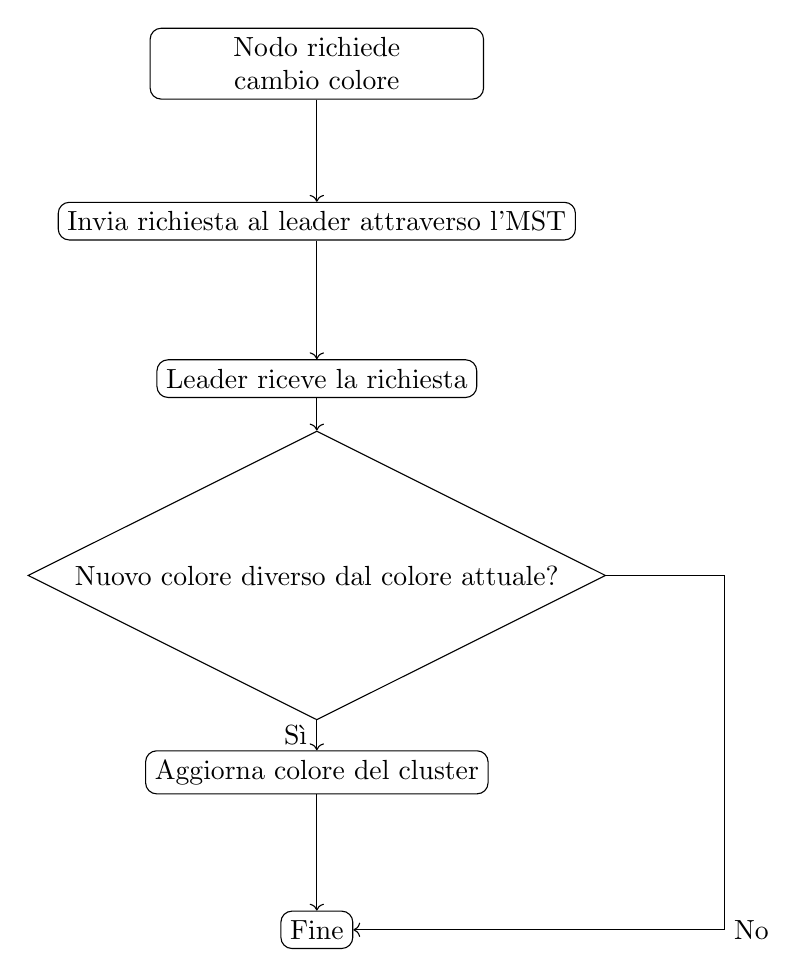
\begin{tikzpicture}[node distance=2cm]
    \node (start) [rectangle, draw, rounded corners, text centered, text width=4cm] {Nodo richiede cambio colore};
    \node (send) [rectangle, draw, rounded corners, below of=start] {Invia richiesta al leader attraverso l'MST};
    \node (receive) [rectangle, draw, rounded corners, below of=send] {Leader riceve la richiesta};
    \node (check) [diamond, draw, aspect=2, below of=receive, yshift=-0.5cm] {Nuovo colore diverso dal colore attuale?};
    \node (update) [rectangle, draw, rounded corners, below of=check, yshift=-0.5cm] {Aggiorna colore del cluster};
    \node (end) [rectangle, draw, rounded corners, below of=update] {Fine};
    \draw [->] (start) -- (send);
    \draw [->] (send) -- (receive);
    \draw [->] (receive) -- (check);
    \draw [->] (check) -- node[anchor=east] {Sì} (update);
    \draw [->] (update) -- (end);
    \draw [->] (check.east) -- ++(1.5cm,0) |- node[anchor=west] {No} (end.east);
\end{tikzpicture}
\caption{Diagramma di flusso dell'Algoritmo di Cambio Colore}
\label{fig:flow_cambio_colore}
\end{figure}




\subsubsection{Considerazioni Finali sulla Soluzione}

La soluzione scelta rappresenta un compromesso efficace tra semplicità, efficienza e robustezza. L'utilizzo dell'MST permette di ottimizzare la comunicazione interna al cluster, mentre la centralizzazione delle decisioni nei leader e la comunicazione tra leader garantiscono una gestione coerente e scalabile delle operazioni a livello di sistema.

\textbf{Vantaggi della Soluzione Proposta}:

\begin{itemize}
    \item \textbf{Efficienza}: L'MST minimizza il numero di messaggi necessari per la comunicazione interna.
    \item \textbf{Scalabilità}: Il sistema è in grado di gestire un grande numero di nodi senza degradare le prestazioni.
    \item \textbf{Robustezza}: L'algoritmo di elezione e la gestione distribuita del leader assicurano la continuità operativa.
    \item \textbf{Consistenza}: La centralizzazione delle decisioni nei leader mantiene lo stato del sistema consistente.
\end{itemize}

\newpage

\section*{TO DO}
\begin{itemize}
    \item gestione failure
    \item spiegare melgio gli algoritmi
    \item spiegare meglio le componenti del sistema => (interfaccia grafica? DB? ..)
\end{itemize}


\end{document}
